\documentclass[presentation]{beamer}
\usepackage{colortbl} 
\usepackage{amsmath}  
\usepackage{float}
\usepackage{pgfplots}
\usepackage{hyperref}
\usepackage{pgfplotstable}
\usepackage{colortbl}
\usepackage{booktabs}
\usepackage{siunitx}
\pgfplotsset{compat=1.18}
\usepackage{caption}
\usepackage{subcaption}
\usepackage{listings}
\usepackage{hyperref}
\hypersetup{
    colorlinks=false,
    pdfborder={0 0 0}
}
\usepackage{biblatex}
\usepackage{tikz}
\usetikzlibrary{arrows.meta, positioning, calc}
\usepackage{tcolorbox}
\usepackage{xcolor}
\usepackage{colortbl}
\usepackage{tabularx}
\usetikzlibrary{arrows.meta, backgrounds, positioning, matrix}
\usetikzlibrary{patterns}


\definecolor{codegreen}{rgb}{0,0.6,0}
\definecolor{codeblue}{rgb}{0,0,0.6}
\definecolor{codegray}{rgb}{0.5,0.5,0.5}

\lstdefinestyle{CStyle}{
    language=C,
    basicstyle=\ttfamily\footnotesize,
    keywordstyle=\color{codeblue},
    commentstyle=\color{codegreen},
    stringstyle=\color{codegray},
    numbers=left,
    numberstyle=\tiny\color{codegray},
    stepnumber=1,
    numbersep=5pt,
    showstringspaces=false,
    tabsize=4,
    captionpos=b,
    breaklines=true,
    breakatwhitespace=false,
    frame=single,
    moredelim=**[is][\lsthighlight]{@}{@}
}

\lstdefinestyle{AsmStyle}{
  language=[x86masm]Assembler,
  basicstyle=\ttfamily\footnotesize,
  keywordstyle=\color{codeblue},
  commentstyle=\color{codegreen},
  stringstyle=\color{codegray},
  numbers=left,
  numberstyle=\tiny\color{codegray},
  stepnumber=1,
  numbersep=5pt,
  showstringspaces=false,
  tabsize=4,
  captionpos=b,
  breaklines=true,
  breakatwhitespace=false,
  frame=single,
  moredelim=**[is][\lsthighlight]{@}{@},
  morekeywords={ldr, str, cmp, csel, b.ge, add, ret, mov, stp, ldp, uxtw}
}

\newcommand{\lsthighlight}{%
  \makebox[0pt][l]{\color{red!10}\rule[-1ex]{\linewidth}{\baselineskip}}}
\newcommand{\armvs}{\texttt{ARMv7} }

\addbibresource{references.bib}

\usefonttheme{structurebold}
\usetheme{Madrid} 
\usecolortheme{seahorse}

\title{Predication and Speculation}%Titel
\subtitle{Compilers for High Performance Computers}%Untertitel
\author{Stefano Petrilli\\ \texttt{stefano.petrilli@upc.edu}\\[1ex] % [1ex] adds vertical space
  Jakob Eberhardt\\ \texttt{jakob.eberhardt@estudiantat.upc.edu}}
%\institute{Universitat Politècnica de Catalunya}
\date{\today{}}
\setbeamertemplate{footline}{
   \leavevmode%
   \hbox{%
   \begin{beamercolorbox}[wd=.333333\paperwidth,ht=2.25ex,dp=1ex,center]{author in head/foot}%
     Stefano Petrilli, Jakob Eberhardt%Kann auch leer sein
   \end{beamercolorbox}%
   \begin{beamercolorbox}[wd=.333333\paperwidth,ht=2.25ex,dp=1ex,center]{title in head/foot}%
     \today{}
   \end{beamercolorbox}%
   \begin{beamercolorbox}[wd=.333333\paperwidth,ht=2.25ex,dp=1ex,right]{date in head/foot}%
     \insertframenumber{} / \inserttotalframenumber\hspace*{2ex} 
   \end{beamercolorbox}}%
   \vskip0pt%
}

\begin{document}
\frame{\titlepage}

\begin{frame}[fragile]{Problem Introduction}
    \begin{lstlisting}[style=CStyle]
void process_data(int *data, int size) {
    for (int i = 0; i < size; i++) {
        if (data[i] < 50) {
            data[i] = 0;
        }
    }
}
\end{lstlisting}
    \captionof{lstlisting}{For \texttt{size=100000000}, we take 1.348 seconds}
    \label{lst:baseline_c} 
\begin{block}{Conditional Codes}
    \begin{itemize}
        \item Concern control flow of the program
        \item Jump to a different instruction based on a condition
        \item May effect performance
    \end{itemize}
\end{block}
\end{frame}

\begin{frame}[fragile]{Instructions have to wait for dependencies}
    \begin{center}
        \resizebox{0.75\textwidth}{!}{
            \begin{lstlisting}[style=AsmStyle]
loop:
    cmp w21, w20                // compare i with size
    b.ge end_loop               // if i >= size, exit loop
@    ldr w0, [x19, w21, UXTW #2] // w0 = data[i] @
@    cmp w0, #50 @
@    b.ge skip_update            // if data[i] >= 50, skip @
@    mov w0, #0                  // w0 = 0  @
    str w0, [x19, w21, UXTW #2] // data[i] = w0
skip_update:
    add w21, w21, #1            // i++
    b loop
\end{lstlisting}
        }
    \end{center}
    
    \vspace{0cm}
    \begin{figure}
        \centering
        \resizebox{0.73\textwidth}{!}{
            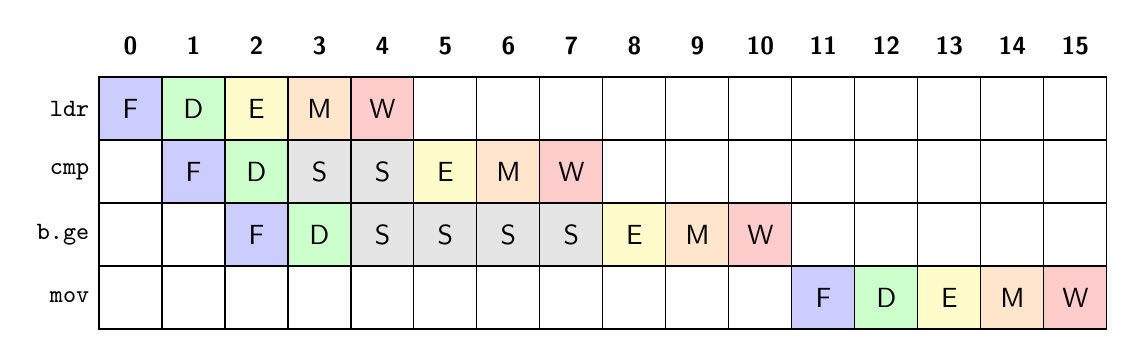
\begin{tikzpicture}[font=\sffamily, scale=0.8]
% Define styles for pipeline stages
\tikzstyle{F} = [fill=blue!20, draw=black, rectangle, minimum width=1cm, minimum height=0.8cm]
\tikzstyle{D} = [fill=green!20, draw=black, rectangle, minimum width=1cm, minimum height=0.8cm]
\tikzstyle{E} = [fill=yellow!20, draw=black, rectangle, minimum width=1cm, minimum height=0.8cm]
\tikzstyle{M} = [fill=orange!20, draw=black, rectangle, minimum width=1cm, minimum height=0.8cm]
\tikzstyle{W} = [fill=red!20, draw=black, rectangle, minimum width=1cm, minimum height=0.8cm]
\tikzstyle{S} = [fill=gray!20, draw=black, rectangle, minimum width=1cm, minimum height=0.8cm]

% Define the number of cycles and instructions
\def\numcycles{15}
\def\numinstr{4}

% Draw the grid
\foreach \i in {1,...,\numinstr} {
    \foreach \j in {0,...,\numcycles} {
        \draw (\j,-\i) rectangle (\j+1,-\i+1);
    }
}

% Label cycles at the top
\foreach \j in {0,...,\numcycles} {
    \node at (\j+0.5,0.5) {\small\textbf{\j}};
}

% Label instructions on the left
\node[anchor=east] at (0,-0.5) {\small \texttt{ldr}};
\node[anchor=east] at (0,-1.5) {\small \texttt{cmp}};
\node[anchor=east] at (0,-2.5) {\small \texttt{b.ge}};
\node[anchor=east] at (0,-3.5) {\small \texttt{mov}};

% Fill in the pipeline stages for each instruction

% Instruction 1 (ldr)
\draw[F] (0,-1) rectangle +(1,1) node[pos=.5] {F};
\draw[D] (1,-1) rectangle +(1,1) node[pos=.5] {D};
\draw[E] (2,-1) rectangle +(1,1) node[pos=.5] {E};
\draw[M] (3,-1) rectangle +(1,1) node[pos=.5] {M};
\draw[W] (4,-1) rectangle +(1,1) node[pos=.5] {W};

% Instruction 2 (cmp)
\draw[F] (1,-2) rectangle +(1,1) node[pos=.5] {F};
\draw[D] (2,-2) rectangle +(1,1) node[pos=.5] {D};
\draw[S] (3,-2) rectangle +(1,1) node[pos=.5] {S};
\draw[S] (4,-2) rectangle +(1,1) node[pos=.5] {S};
\draw[E] (5,-2) rectangle +(1,1) node[pos=.5] {E};
\draw[M] (6,-2) rectangle +(1,1) node[pos=.5] {M};
\draw[W] (7,-2) rectangle +(1,1) node[pos=.5] {W};

% Instruction 3 (b.ge)
\draw[F] (2,-3) rectangle +(1,1) node[pos=.5] {F};
\draw[D] (3,-3) rectangle +(1,1) node[pos=.5] {D};
\draw[S] (4,-3) rectangle +(1,1) node[pos=.5] {S};
\draw[S] (5,-3) rectangle +(1,1) node[pos=.5] {S};
\draw[S] (6,-3) rectangle +(1,1) node[pos=.5] {S};
\draw[S] (7,-3) rectangle +(1,1) node[pos=.5] {S};
\draw[E] (8,-3) rectangle +(1,1) node[pos=.5] {E};
\draw[M] (9,-3) rectangle +(1,1) node[pos=.5] {M};
\draw[W] (10,-3) rectangle +(1,1) node[pos=.5] {W};


% Instruction 4 (mov w0, #0)
\draw[F] (11,-4) rectangle +(1,1) node[pos=.5] {F};
\draw[D] (12,-4) rectangle +(1,1) node[pos=.5] {D};
\draw[E] (13,-4) rectangle +(1,1) node[pos=.5] {E};
\draw[M] (14,-4) rectangle +(1,1) node[pos=.5] {M};
\draw[W] (15,-4) rectangle +(1,1) node[pos=.5] {W};

% % Add legends for pipeline stages
% \matrix [draw, below right] at (14,-0.5) {
%   \node [F] {F}; & \node [anchor=west] {Fetch}; \\
%   \node [D] {D}; & \node [anchor=west] {Decode}; \\
%   \node [E] {E}; & \node [anchor=west] {Execute}; \\
%   \node [M] {M}; & \node [anchor=west] {Memory}; \\
%   \node [W] {W}; & \node [anchor=west] {Write Back}; \\
%   \node [S] {S}; & \node [anchor=west] {Stall}; \\
% };

\end{tikzpicture}
 % Include the figure from an external file.
        }
        \caption{We need to wait for \texttt{data[i]} to be written back to \texttt{w0} for the comparison. We also need to wait for \texttt{b.ge} to finish to know which instruction to fetch next}
        \label{fig:pipeline-stages}
    \end{figure}
\end{frame}


\begin{frame}[fragile]{Instructions have to wait for dependencies}
    \begin{block}{Problem}
        \begin{itemize}
            \item We have to wait for \texttt{data[i]} to be loaded
            \item We cannot exploit available resources 
            \item We do not know which instruction to fetch next
            \item Pipeline stalls, IPC$\downarrow$
            \item \textbf{We need to reduce the cost of conditional branching}
        \end{itemize}
        \end{block}
    \vspace{0cm}
    \begin{figure}
        \centering
        \resizebox{\linewidth}{!}{
            
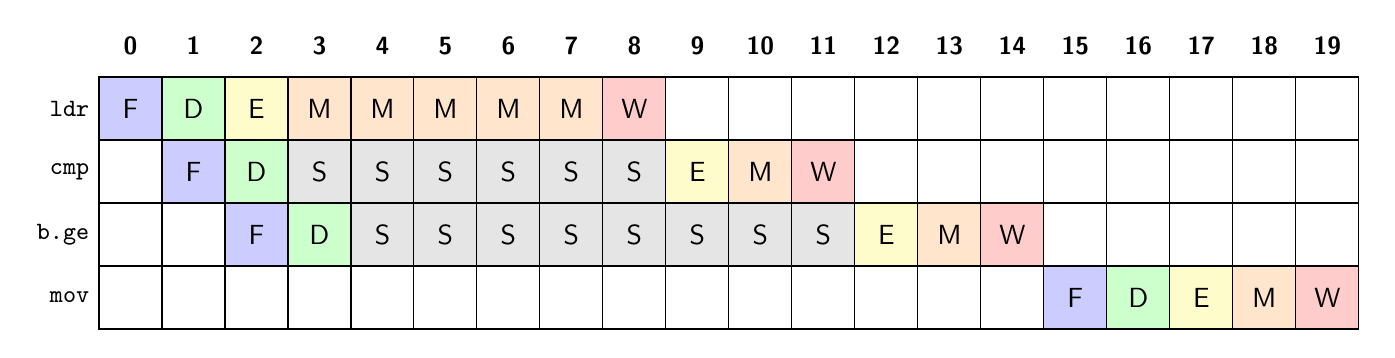
\begin{tikzpicture}[font=\sffamily, scale=0.8]
% Define styles for pipeline stages
\tikzstyle{F} = [fill=blue!20, draw=black, rectangle, minimum width=1cm, minimum height=0.8cm]
\tikzstyle{D} = [fill=green!20, draw=black, rectangle, minimum width=1cm, minimum height=0.8cm]
\tikzstyle{E} = [fill=yellow!20, draw=black, rectangle, minimum width=1cm, minimum height=0.8cm]
\tikzstyle{M} = [fill=orange!20, draw=black, rectangle, minimum width=1cm, minimum height=0.8cm]
\tikzstyle{W} = [fill=red!20, draw=black, rectangle, minimum width=1cm, minimum height=0.8cm]
\tikzstyle{S} = [fill=gray!20, draw=black, rectangle, minimum width=1cm, minimum height=0.8cm]

% Define the number of cycles and instructions
\def\numcycles{19}
\def\numinstr{4}

% Draw the grid
\foreach \i in {1,...,\numinstr} {
    \foreach \j in {0,...,\numcycles} {
        \draw (\j,-\i) rectangle (\j+1,-\i+1);
    }
}

% Label cycles at the top
\foreach \j in {0,...,\numcycles} {
    \node at (\j+0.5,0.5) {\small\textbf{\j}};
}

% Label instructions on the left
\node[anchor=east] at (0,-0.5) {\small \texttt{ldr}};
\node[anchor=east] at (0,-1.5) {\small \texttt{cmp}};
\node[anchor=east] at (0,-2.5) {\small \texttt{b.ge}};
\node[anchor=east] at (0,-3.5) {\small \texttt{mov}};

% Fill in the pipeline stages for each instruction

% Instruction 1 (ldr)
\draw[F] (0,-1) rectangle +(1,1) node[pos=.5] {F};
\draw[D] (1,-1) rectangle +(1,1) node[pos=.5] {D};
\draw[E] (2,-1) rectangle +(1,1) node[pos=.5] {E};
\draw[M] (3,-1) rectangle +(1,1) node[pos=.5] {M};
\draw[M] (4,-1) rectangle +(1,1) node[pos=.5] {M};
\draw[M] (5,-1) rectangle +(1,1) node[pos=.5] {M};
\draw[M] (6,-1) rectangle +(1,1) node[pos=.5] {M};
\draw[M] (7,-1) rectangle +(1,1) node[pos=.5] {M};
\draw[W] (8,-1) rectangle +(1,1) node[pos=.5] {W};

% Instruction 2 (cmp)
\draw[F] (1,-2) rectangle +(1,1) node[pos=.5] {F};
\draw[D] (2,-2) rectangle +(1,1) node[pos=.5] {D};
\foreach \c in {3,...,8} {
    \draw[S] (\c,-2) rectangle +(1,1) node[pos=.5] {S};
}
\draw[E] (9,-2) rectangle +(1,1) node[pos=.5] {E};
\draw[M] (10,-2) rectangle +(1,1) node[pos=.5] {M};
\draw[W] (11,-2) rectangle +(1,1) node[pos=.5] {W};

% Instruction 3 (b.ge)
\draw[F] (2,-3) rectangle +(1,1) node[pos=.5] {F};
\draw[D] (3,-3) rectangle +(1,1) node[pos=.5] {D};
\foreach \c in {4,...,11} {
    \draw[S] (\c,-3) rectangle +(1,1) node[pos=.5] {S};
}
\draw[E] (12,-3) rectangle +(1,1) node[pos=.5] {E};
\draw[M] (13,-3) rectangle +(1,1) node[pos=.5] {M};
\draw[W] (14,-3) rectangle +(1,1) node[pos=.5] {W};

% Instruction 4 (mov)
\draw[F] (15,-4) rectangle +(1,1) node[pos=.5] {F};
\draw[D] (16,-4) rectangle +(1,1) node[pos=.5] {D};
\draw[E] (17,-4) rectangle +(1,1) node[pos=.5] {E};
\draw[M] (18,-4) rectangle +(1,1) node[pos=.5] {M};
\draw[W] (19,-4) rectangle +(1,1) node[pos=.5] {W};

\end{tikzpicture}

        }
        \caption{A Cache miss may effect the pipeline even more.}
        \label{fig:pipeline-diagram}
    \end{figure}

\end{frame}

\begin{frame}{Methods}
\begin{center}

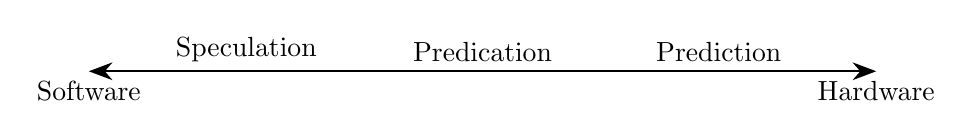
\begin{tikzpicture}[align=center]

\draw[arrows={Stealth[length=3mm]-Stealth[length=3mm]}, thick] (0,0) -- (10,0);

% Place labels at the ends
\node[below] at (0,0) {Software};
\node[below] at (10,0) {Hardware};

\node[above] at (2,0) {Speculation};
\node[above] at (5,0) {Predication};
\node[above] at (8,0) {Prediction};

\end{tikzpicture}
\end{center}
\begin{itemize}
    \item \textbf{Speculation}
        \begin{itemize}
            \item Speculate about control flow at run time while compiling
            \item Generate additional code, e.g., compensation code 
        \end{itemize}
    \item \textbf{Predication}
        \begin{itemize}
            \item Execute multiple branches
            \item Select correct result when condition arrives
            \item Requires special instructions, e.g., \texttt{cmov}
        \end{itemize}
    \item \textcolor{gray}{\textbf{Prediction}} 
        \begin{itemize}
            \item \textcolor{gray}{Try to predict control flow during run time}
            \item \textcolor{gray}{Using a hardware structure such as a branch predictor}
        \end{itemize}
\end{itemize}

\end{frame}

\begin{frame}{Speculation}
    \begin{block}{Definition}
    "An instruction is \textit{speculatively} executed if it is moved above a conditional branch that it is control dependent upon"~\cite{chang95}
    \end{block}
    \begin{itemize}
        \item \textbf{Compiler-controlled}
            \begin{itemize}
              \item Speculate about real control flow
              \item Try to enable other optimization opportunities
        \end{itemize}
        \item \textbf{Control Speculation}
        \begin{itemize}
               \item Execute instructions before control flow was determined 
        \end{itemize}
        \item \textbf{Data Speculation}
        \begin{itemize}
            \item Execute instructions with potentially wrong data 
        \end{itemize}
    \end{itemize}
\end{frame}

\begin{frame}{Exceptions}
        \begin{table}
\label{tab:save_unsafe}
    \begin{tabularx}{\linewidth}{|>{\centering\arraybackslash}c|X|X|}
    \hline
    \rowcolor{gray!50}
    \textbf{Type} & \textbf{Behavior} & \textbf{Example} \\ \hline
    \textit{safe} & Never causes an exception to a dominating block & Register-to-register operations \\ \hline
    \textit{unsafe} & Can always cause an exception to a dominating block & Loads, certain floating-point instructions \\
    \hline
    \end{tabularx}
\end{table}

\end{frame}
    
\begin{frame}[fragile]
\frametitle{Predicated Execution without Branching}

\begin{lstlisting}[style=AsmStyle]
loop_predicated:
    cmp w21, w20                    // compare i with size
    b.ge end_predicated             // if i >= size, exit loop

    ldr w0, [x19, w21, UXTW #2]     // w0 = data[i]
    cmp w0, #50
    csel w0, wzr, w0, lt            // if w0 < 50, w0 = 0; else w0 = w0
    str w0, [x19, w21, UXTW #2]     // data[i] = w0

    add w21, w21, #1                // i++
    b loop_predicated
\end{lstlisting}

\end{frame}

\begin{frame}[fragile]
\frametitle{Speculative Execution with Branching}

\begin{lstlisting}[style=AsmStyle]
loop_speculative:
    cmp w21, w20                // compare i with size
    b.ge end_speculative        // if i >= size, exit loop

    ldr w0, [x19, w21, UXTW #2] // w0 = data[i]
    cmp w0, #50
    b.ge skip_update            // if data[i] >= 50, skip update
    mov w0, #0                  // w0 = 0
    str w0, [x19, w21, UXTW #2] // data[i] = w0
skip_update:
    add w21, w21, #1            // i++
    b loop_speculative
\end{lstlisting}
\end{frame}



% \begin{frame}{Introduction}
\begin{tikzpicture}[remember picture, overlay]
  \node[anchor=north east, inner sep=0pt, yshift=-1cm, xshift=-0.5cm] at (current page.north east) {
    \includegraphics[width=2cm]{assets/placeholder.png}
  };
  \node[anchor=south east, inner sep=0pt, yshift=2cm, xshift=-0.5cm] at (current page.south east) {
    \includegraphics[width=2cm]{assets/placeholder.png}
  };
\end{tikzpicture}

\begin{itemize}
    \item Solves the linear heat conduction equation in 2D
    \item Application consists of low-complexity kernels
    \begin{itemize}
        \item Conjugate Gradient, Chebyshev, Jacobi
    \end{itemize}
    \item Many implementations are available
    \begin{itemize}
        \item \textbf{Fortran with MPI}
        \item OpenCL, CUDA, Petsc, Trilinos, Hypre
    \end{itemize}
    \item Source code: \href{https://github.com/UK-MAC/TeaLeaf}{github.com/UK-MAC/TeaLeaf} \cite{tearepo}

\end{itemize}
\end{frame}
% \begin{frame}{List with Figure}
\begin{columns}
    \begin{column}{0.48\textwidth}
        \begin{itemize}
            \item First
            \item Second
            \item Third 
        \end{itemize}
    \end{column}
    \begin{column}{0.48\textwidth}
        \centering
        \includegraphics[width=\linewidth]{assets/placeholder.png}
        \captionof{figure}{Caption}
    \end{column}
\end{columns}
\end{frame}

% \begin{frame}{List with Two Figures}
\begin{figure}
    \centering
    \begin{minipage}{0.48\textwidth}
        \begin{itemize}
            \item First Bullet Point
            \item Second Bullet Point
            \item Third Bullet Point
            \item Fourth Bullet Point
            \item Fifth Bullet Point
        \end{itemize}
    \end{minipage}
    \begin{minipage}{0.48\textwidth}
        \centering
        \includegraphics[width=0.4\linewidth]{assets/placeholder.png}
        \caption{First Image Caption}
        \vspace{10pt}
        \includegraphics[width=0.4\linewidth]{assets/placeholder.png}
        \caption{Second Image Caption}
    \end{minipage}
\end{figure}
\end{frame}

% \begin{frame}{Block and Lsit}
\begin{block}{Block Title}
For an order $i$:
        \begin{itemize}
            \item Also consider other attributes:
            $$\frac{\mathit{profit}_i (\mathit{max\_deliver}_i - \mathit{min\_deliver}_i)}{(\mathit{length}_i \cdot \mathit{surface}_i)}$$
        \end{itemize}
\end{block}

\begin{itemize}
        \item Objective function value: 126 
        \item \textbf{Optimality gap: 23\%} 
        \end{itemize}
\end{frame}
% \begin{frame}{Two Images Side by Side}
\begin{figure}
    \centering
    % First image on the left
    \begin{minipage}{0.48\textwidth}
        \centering
        \includegraphics[width=\linewidth]{assets/placeholder.png}
        \caption{First Image Caption}
    \end{minipage}\hfill
    % Second image on the right
    \begin{minipage}{0.48\textwidth}
        \centering
        \includegraphics[width=\linewidth]{assets/placeholder.png}
        \caption{Second Image Caption}
    \end{minipage}
\end{figure}
\end{frame}

% \begin{frame}{Three Side-by-Side}
\begin{figure}
    \centering
    \begin{minipage}{0.32\textwidth}
        \centering
        \includegraphics[width=\linewidth]{assets/placeholder.png} % Adjust path as needed
        \caption{Caption 1}
    \end{minipage}\hfill
    \begin{minipage}{0.32\textwidth}
        \centering
        \includegraphics[width=\linewidth]{assets/placeholder.png} % Adjust path as needed
        \caption{Caption 1}
    \end{minipage}\hfill
    \begin{minipage}{0.32\textwidth}
        \centering
        \includegraphics[width=\linewidth]{assets/placeholder.png} % Adjust path as needed
        \caption{Caption 1}
    \end{minipage}
\end{figure}
\end{frame}

% \begin{frame}{Plot}
    \centering
    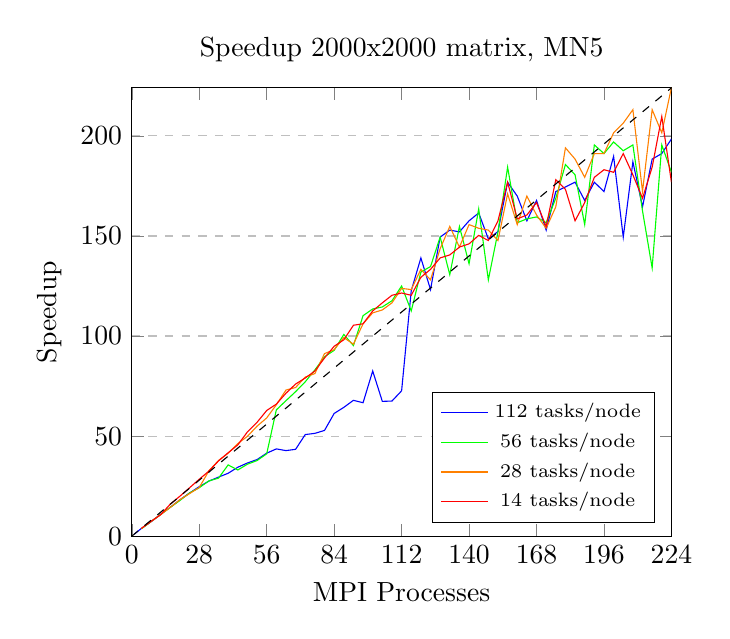
\begin{tikzpicture}
    \begin{axis}[
        title={Speedup 2000x2000 matrix, MN5},
        xlabel={MPI Processes},
        ylabel={Speedup},
        xmin=0, xmax=224,
        ymin=0, ymax=224,
        xtick={0,20,40,60,80,100,120,140,160,180,224},
        xtick={0,28,56,84,112,140,168, 196, 224},
        legend pos=south east,
        legend style={font=\scriptsize},
        ymajorgrids=true,
        grid style=dashed,
    ]
    
    \addplot[color=blue] coordinates {
    (1, 1.0)
    (4, 3.89)
    (8, 7.21)
    (12, 10.92)
    (16, 14.46)
    (20, 18.21)
    (24, 21.58)
    (28, 24.74)
    (32, 27.51)
    (36, 29.51)
    (40, 31.44)
    (44, 34.44)
    (48, 36.57)
    (52, 38.29)
    (56, 41.47)
    (60, 43.62)
    (64, 42.76)
    (68, 43.41)
    (72, 50.78)
    (76, 51.38)
    (80, 52.85)
    (84, 61.32)
    (88, 64.36)
    (92, 67.89)
    (96, 66.67)
    (100, 82.54)
    (104, 67.36)
    (108, 67.53)
    (112, 72.63)
    (116, 122.64)
    (120, 139.04)
    (124, 123.22)
    (128, 149.43)
    (132, 152.94)
    (136, 152.05)
    (140, 157.58)
    (144, 161.49)
    (148, 148.57)
    (152, 152.2)
    (156, 176.87)
    (160, 169.93)
    (164, 157.58)
    (168, 167.74)
    (172, 152.94)
    (176, 172.19)
    (180, 174.50)
    (184, 176.87)
    (188, 167.74)
    (192, 176.87)
    (196, 172.19)
    (200, 189.78)
    (204, 149.43)
    (208, 187.05)
    (212, 164.56)
    (216, 188.41)
    (220, 191.18)
    (224, 198.47)
    };
    \addlegendentry{112 tasks/node}
    
    \addplot[color=green] coordinates {
    (4, 3.70)
    (8, 7.34)
    (12, 10.85)
    (16, 14.44)
    (20, 17.87)
    (24, 21.61)
    (28, 24.21)
    (32, 27.63)
    (36, 28.99)
    (40, 35.62)
    (44, 33.08)
    (48, 35.96)
    (52, 37.79)
    (56, 41.14)
    (60, 63.11)
    (64, 67.71)
    (68, 72.22)
    (72, 77.15)
    (76, 83.07)
    (80, 89.66)
    (84, 92.86)
    (88, 100.78)
    (92, 95.24)
    (96, 110.17)
    (100, 113.54)
    (104, 114.54)
    (108, 117.65)
    (112, 125.00)
    (116, 112.55)
    (120, 131.98)
    (124, 134.72)
    (128, 149.43)
    (132, 130.65)
    (136, 154.76)
    (140, 136.13)
    (144, 163.52)
    (148, 128.08)
    (152, 152.05)
    (156, 184.40)
    (160, 156.63)
    (164, 158.54)
    (168, 159.51)
    (172, 156.63)
    (176, 168.83)
    (180, 185.71)
    (184, 180.56)
    (188, 155.69)
    (192, 195.49)
    (196, 191.18)
    (200, 196.97)
    (204, 192.59)
    (208, 195.49)
    (212, 162.50)
    (216, 134.02)
    (220, 195.49)
    (224, 181.82)
    };
    \addlegendentry{56 tasks/node}
    
    \addplot[color=orange] coordinates {
    (4, 3.87)
    (8, 7.30)
    (12, 10.82)
    (16, 14.37)
    (20, 18.27)
    (24, 21.29)
    (28, 24.34)
    (32, 32.62)
    (36, 37.79)
    (40, 41.47)
    (44, 46.26)
    (48, 49.90)
    (52, 54.97)
    (56, 59.09)
    (60, 65.66)
    (64, 73.03)
    (68, 74.29)
    (72, 79.51)
    (76, 81.25)
    (80, 91.23)
    (84, 93.19)
    (88, 99.24)
    (92, 95.94)
    (96, 106.12)
    (100, 111.59)
    (104, 113.04)
    (108, 116.59)
    (112, 123.81)
    (116, 123.22)
    (120, 133.33)
    (124, 128.08)
    (128, 143.65)
    (132, 154.76)
    (136, 144.44)
    (140, 155.69)
    (144, 153.85)
    (148, 152.94)
    (152, 147.73)
    (156, 171.05)
    (160, 155.69)
    (164, 169.93)
    (168, 160.49)
    (172, 153.85)
    (176, 164.56)
    (180, 194.03)
    (184, 188.41)
    (188, 179.31)
    (192, 191.18)
    (196, 191.18)
    (200, 201.55)
    (204, 206.35)
    (208, 213.11)
    (212, 172.19)
    (216, 213.11)
    (220, 201.55)
    (224, 224.14)
    
    };
    \addlegendentry{28 tasks/node}
    
    
    
    \addplot[color=red] coordinates {
    (4, 3.89)
    (8, 7.43)
    (12, 10.75)
    (16, 16.05)
    (20, 20.00)
    (24, 24.21)
    (28, 28.45)
    (32, 32.50)
    (36, 37.63)
    (40, 41.67)
    (44, 45.61)
    (48, 52.10)
    (52, 56.89)
    (56, 62.80)
    (60, 65.99)
    (64, 71.43)
    (68, 76.02)
    (72, 79.03)
    (76, 82.54)
    (80, 89.04)
    (84, 94.89)
    (88, 98.11)
    (92, 105.4)
    (96, 106.12)
    (100, 112.55)
    (104, 116.59)
    (108, 120.37)
    (112, 121.50)
    (116, 120.37)
    (120, 129.35)
    (124, 133.33)
    (128, 139.04)
    (132, 140.54)
    (136, 144.44)
    (140, 146.07)
    (144, 150.29)
    (148, 147.73)
    (152, 157.58)
    (156, 176.87)
    (160, 158.54)
    (164, 160.49)
    (168, 166.67)
    (172, 154.76)
    (176, 178.08)
    (180, 173.33)
    (184, 157.58)
    (188, 166.67)
    (192, 179.31)
    (196, 183.10)
    (200, 181.82)
    (204, 191.18)
    (208, 180.56)
    (212, 168.83)
    (216, 184.40)
    (220, 209.68)
    (224, 176.87)
    
    };
    \addlegendentry{14 tasks/node}
    
    \addplot[color=black, dashed, domain=0:224] {x};
    
    
    
    
    \end{axis}
    \end{tikzpicture}
\end{frame}


% \newcommand{\stencilpt}[4][]{\node[draw,inner sep=0.1em,minimum size=1.2cm,font=\small,#1] at (#2) (#3) {#4}}
\begin{frame}{Stencil}   
    \centering
    \begin{tikzpicture}
      \stencilpt[fill=orange!30]{-1.5,0}{i-1}{$(i, j-1)$}; % Left neighbor
      \stencilpt[fill=blue!30]{0,0}{i}{$(i, j)$}; % Central point
      \stencilpt[fill=orange!30]{1.5,0}{i+1}{$(i, j+1)$}; % Right neighbor
      \stencilpt[fill=orange!30]{0,1.5}{j+1}{$(i-1, j)$}; % Top neighbor
      \stencilpt[fill=orange!30]{0,-1.5}{j-1}{$(i+1, j)$}; % Bottom neighbor
    
      \draw (i) -- (i-1)
            (i) -- (i+1)
            (i) -- (j+1)
            (i) -- (j-1);
    \end{tikzpicture}
\end{frame}

% \begin{frame}{Two Images Side by Side}
\begin{figure}
    \centering
    % First image on the left
    \begin{minipage}{0.48\textwidth}
        \centering
        \includegraphics[width=\linewidth]{assets/placeholder.png}
        \caption{First Image Caption}
    \end{minipage}\hfill
    % Second image on the right
    \begin{minipage}{0.48\textwidth}
        \centering
        \includegraphics[width=\linewidth]{assets/placeholder.png}
        \caption{Second Image Caption}
    \end{minipage}
\end{figure}
\end{frame}

% \begin{frame}[fragile]{Hello World in MPI}
\begin{lstlisting}[language=C, basicstyle=\small\ttfamily, keywordstyle=\color{blue}]
#include <mpi.h>
#include <stdio.h>

int main(int argc, char** argv) {
    MPI_Init(&argc, &argv);
    int world_rank;
    MPI_Comm_rank(MPI_COMM_WORLD, &world_rank);
    printf("Hello world from rank %d\n", world_rank);
    MPI_Finalize();
    return 0;
}
\end{lstlisting}
\captionof{lstlisting}{Hello World program using MPI.}
\label{lst:mpi_hello_world} 
\end{frame}




\begin{frame}[allowframebreaks]{References \& Questions}
    \printbibliography
\end{frame}
\end{document}
